\documentclass[a4paper,12pt]{report}
\usepackage[left=2cm,right=2cm,top=2cm,bottom=2cm]{geometry}
\usepackage[utf8]{inputenc}
\usepackage{graphicx}
\usepackage{eso-pic}
\usepackage{transparent}
\usepackage{xcolor}
\usepackage{floatrow}
\usepackage{tabularx}
\usepackage{listings}
\usepackage{caption}
\usepackage{amsmath}

\newcommand{\LogoPath}{RUET_logo.png}

\definecolor{odp-background}{RGB}{40, 44, 52}
\definecolor{odp-text}{RGB}{171, 178, 191}
\definecolor{odp-keyword}{RGB}{249, 38, 114}
\definecolor{odp-comment}{RGB}{98, 114, 164}
\definecolor{odp-string}{RGB}{152, 195, 121}
\definecolor{odp-number}{RGB}{174, 129, 255}
\definecolor{odp-function}{RGB}{189, 147, 249}
\definecolor{odp-header}{RGB}{173, 216, 230}

\lstdefinestyle{cppstyle}{
    language=C++,
    basicstyle=\color{odp-text}\ttfamily\small,
    keywordstyle=\color{odp-keyword},
    commentstyle=\color{odp-comment},
    stringstyle=\color{odp-string},
    numbers=left,
    numberstyle=\tiny\color{odp-number},
    stepnumber=1,
    numbersep=5pt,
    backgroundcolor=\color{gray!5},
    frame=single,
    rulecolor=\color{odp-text},
    breaklines=true,
    breakatwhitespace=true,
    tabsize=4,
    moredelim=[s][\color{odp-header}]{\#include\ <}{>}, % Header files included in #include <>
    otherkeywords={!,!=,~,$,*,\&,\%,:,\#, ifndef, define, endif, include},
    emph={!,!=,~,$,*,\&,\%,:,\#},
    emphstyle=\color{odp-function}
}

\begin{document}
\begin{titlepage}
    \begin{center}

        \AddToShipoutPicture*{\put(0.125\paperwidth,0.125\paperheight){
                \transparent{0.1}
                \includegraphics*[width=0.75\paperwidth,height=0.75\paperheight,keepaspectratio]{RUET_logo.png}%
            }
        }
        \textbf{\textcolor{yellow}{\rmfamily Haven's Light is Our Guide}}

        \begin{figure}[h]
            \transparent{0.8}
            \centering
            \includegraphics[width=0.3\textwidth]{\LogoPath}
        \end{figure}

        \vspace*{0in}
        \Large
        \textbf{\mbox{Rajshahi University of Engineering \& Technology}}
        \large
        \textbf{\mbox{\textcolor{blue}{Department of Computer Science \& Engineering}}}

        \vfill
        \Huge
        \textbf{\mbox{Lab Report}}
        \vfill

        \begin{table}[h]
            \centering
            \begin{tabularx}{0.7\paperwidth}{|c|X|}
                \hline
                \textbf{Course Code:}     & CSE 2204                                                   \\
                \hline
                \textbf{Course Title:}    & Numerical Methods Sessional                                \\
                \hline
                \textbf{Experiment No:}   & 02                                                         \\
                \hline
                \textbf{Experiment Name:} & Solving Equations using Iteration and Newton-Rapson Method \\
                \hline
            \end{tabularx}%
        \end{table}

        \vspace{0.5in}
        \textbf{Date:} \\
        \today

        \vfill

        \begin{table}[h]
            \centering
            \begin{tabularx}{0.7\paperwidth}{|X|X|}
                \hline
                Submitted By:               & Submitted To:                                    \\
                \hline
                Name: Md. Abdullah Al Mamun & Shyla Afroge                                     \\
                \hline
                Section: A                  & Assistant Professor                              \\
                \hline
                Roll No: 2003028            & Computer Science \& Engineering                  \\
                \hline
                Year: 2nd Year Odd Semester & Rajshahi University of Engineering \& Technology \\
                \hline
            \end{tabularx}
        \end{table}
    \end{center}
\end{titlepage}

\section*{Experiment No: 02}
\section*{Experiment Name: \small Solving Equations using Iteration and Newton-Rapson Method}
\section*{Theory:}

\subsection*{Iteration Method:}
\qquad Iteration is a fundamental concept in mathematics and numerical methods, involving the process of repeatedly applying a rule or procedure to achieve a desired outcome. In the context of numerical analysis, iteration is commonly used to approximate solutions to equations, particularly when analytical solutions are challenging or impossible to find. The iterative process starts with an initial guess and refines it through successive iterations until a sufficiently accurate solution is obtained.

\subsection*{Algorithm:}
\begin{enumerate}
    \item Initial Guess: Begin with an initial guess or estimate for the solution.
    \item Iterative Process: Apply a rule or procedure to refine the estimate through successive iterations.
    \item Convergence Criteria: Continue the iterations until a specified convergence criterion is met, indicating that the solution is sufficiently accurate.
\end{enumerate}

\subsection*{Newton-Raphson Method:}
\qquad The Newton-Raphson Method is a powerful iterative technique for finding successively better approximations to the roots of a real-valued function. It is based on linear approximation and tangent lines. Starting with an initial guess \(x_0\), the method iteratively refines the approximation using the formula \(x_{n+1} = x_n - \frac{f(x_n)}{f'(x_n)}\), where \(f(x)\) is the function and \(f'(x)\) is its derivative. The method converges rapidly when the initial guess is close to the actual root, making it an efficient tool for root-finding. However, it may fail to converge or converge to an undesired root under certain conditions or if the function has peculiar characteristics. Despite these considerations, the Newton-Raphson Method is widely utilized in various fields for its speed and effectiveness in finding solutions to nonlinear equations.

\subsection*{Algorithm:}
\begin{enumerate}
    \item Initial Guess: Start with an initial guess \(x_0\) for the root.
    \item Iterative Formula: Apply the iterative formula \(x_{n+1} = x_n - \frac{f(x_n)}{f'(x_n)}\), where \(f(x)\) is the function and \(f'(x)\) is its derivative.
    \item Successive Refinement: Repeat the iterative process to successively refine the approximation to the root.
    \item Convergence Criteria: Continue the iterations until a specified convergence criterion is met, indicating that the root approximation is sufficiently accurate.
\end{enumerate}

\section*{Program:}

\begin{lstlisting}[style=cppstyle, caption={Newton-Rapson Method}, label={lst:cppcode}, basicstyle=\fontsize{10}{11}\selectfont\ttfamily]
    double newtonRapsonMethod(double x, double error)
    {
        double x1 = x - function(x) / functionDerivative(x);
        double x2 = x1 - function(x1) / functionDerivative(x1);
    
        cout << "x0: " << x << "\tx1: " << x1 << "\n";
    
        int i = 1;
        while (abs(x2 - x1) > error)
        {
            x1 = x2;
            x2 = x1 - function(x1) / functionDerivative(x1);
            cout << "x" << i << ": " << x1 << "\tx" << (i + 1) << ": " << x2 << "\n";
            i++;
        }
    
        return x2;
    }
\end{lstlisting}

\begin{lstlisting}[style=cppstyle, caption={Iteration Method}, label={lst:cppcode}, basicstyle=\fontsize{10}{11}\selectfont\ttfamily]
    double phiFunction(double x, int coeff[], int degree)
    {
        double sum = 0;
        for (int i = 0; i <= degree; i++)
        {
            sum += coeff[i] * pow(x, i);
        }
        return sum;
    }
    
    double iterarionMethod(double x, double error)
    {
        int degree;
        cout << "Enter degree for phi function: ";
        cin >> degree;
        int coeff[degree + 1];
        cout << "Enter " << degree + 1 << " Coefficients: ";
        for (int i = 0; i <= degree; i++)
            cin >> coeff[i];
    
        double x1 = phiFunction(x, coeff, degree);
        double x2 = phiFunction(x1, coeff, degree);
    
        while (abs(x2 - x1) > error)
        {
            x1 = x2;
            x2 = phiFunction(x1, coeff, degree);
            cout << "x1: " << x1 << "\tx2: " << x2 << "\n";
        }
    
        return x2;
    }
\end{lstlisting}

\begin{lstlisting}[style=cppstyle, caption={functionInput.h helper file}, label={lst:cppcode}, basicstyle=\fontsize{10}{11}\selectfont\ttfamily]
    #ifndef FUNCTIONINPUT_H
    #define FUNCTIONINPUT_H
    #include <iostream>
    #include <cmath>
    
    using namespace std;
    
    int degree;
    int *coefficients = new int[degree + 1];
    
    void takeInputForFunction()
    {
        int deg;
        cout << "Enter the degree of the polynomial: ";
        cin >> deg;
        int *coef = new int[deg + 1];
        cout << "Enter " << deg + 1 << " coefficients of the polynomial: ";
        for (int i = 0; i <= deg; i++)
            cin >> coef[i];
        delete[] coefficients; // free the previously allocated memory
        coefficients = coef;
        degree = deg;
    }
    
    double function(double x)
    {
        double sum = 0;
        for (int i = 0; i <= degree; i++)
        {
            sum += coefficients[i] * pow(x, i);
        }
        return sum;
    }
    
    double functionDerivative(double x)
    {
        double sum = 0;
        for (int i = 1; i <= degree; i++)
            sum += i * coefficients[i] * pow(x, i - 1);
        return sum;
    }
    
    #endif // !FUNCTIONINPUT_H
\end{lstlisting}

\begin{lstlisting}[style=cppstyle, caption={Main Program}, label={lst:cppcode}, basicstyle=\fontsize{10}{11}\selectfont\ttfamily]
    #include <iostream>
    #include "functionInput.h"
    using namespace std;
    
    int main()
    {
        takeInputForFunction();
        double a;
    
        cout << "Enter guess: ";
        cin >> a;
    
        cout << "\n1. Newton Rapson Method\n2. Iteration Method\n";
        cout << "Choose the method you want to use: ";
    
        int choice;
        cin >> choice;
        switch (choice)
        {
            {
            case 1:
            {
                double sol = newtonRapsonMethod(a, 0.0001);
                cout << "The solution using Newton-Rapson Method: " << sol << endl;
                break;
            }
    
            case 2:
            {
                double sol = iterarionMethod(a, 0.0001);
                cout << "The solution using Iteration Method: " << sol << endl;
                break;
            }
    
            default:
                break;
            }
        }
    }
\end{lstlisting}

\section*{Result:}
\qquad The Newton-Raphson Method and the Iteration Method are both iterative techniques used for approximating solutions to mathematical problems. The Newton-Raphson Method utilizes function derivatives for rapid convergence, especially when initial guesses are close to roots, but it may be sensitive to specific conditions. In contrast, the Iteration Method is a more general approach, suitable for a wide range of functions, although it tends to converge more slowly. The choice between these methods depends on the specific characteristics of the problem and the quality of the initial guess.

\begin{figure}[H]
    \centering
    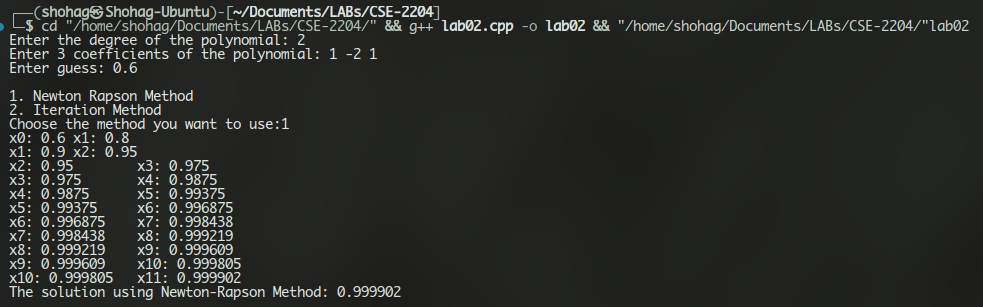
\includegraphics[width=\textwidth]{result.png}
    \caption{Output of the Program}
    \label{fig:result}
\end{figure}

\end{document}